\chapter{Livermore Solver for Ordinary Differential Equations (LSODE)}
\label{app:lsode}

\section{Overview}

The Livermore Solver for Ordinary Differential Equations (LSODE) is an
adaptive step integrator.  It computes its preferred integration step
internally, independently of the step-size requested by
the simulation engine.  In order to obtain the state at the externally-defined
(i.e. by the simulation engine) time-step boundary, LSODE performs an
iteration using the two states (at the internally-generated time-step
boundaries) on either side of the requested time.

This LSODE
implementation is adapted from the fortran DLSODE
package~\cite{code:dlsode} (local copy provided for reference).
Cross-references to
the original code are included as comments in the code throughout this
implementation.

The adaptation is driven by two key requirements:
\begin{enumerate}
\item
Translation from Fortran to C++
\item
Architectural transformation to work from within a simulation engine (e.g.
Trick).
\end{enumerate}

The latter of these requirements deserves some elaboration to illustrate
the fundamentally different paradigms under which this implementation and the
original DLSODE implementation operate.
\begin{itemize}
\item The DLSODE fortran code~\cite{code:dlsode}
is used as a standalone routine.
In such a paradigm, the user calls the integrator, then
external calls are made
-- from within the integrator --
to compute
derivatives along the integration path.
The variables are then integrated
according to incoming derivative values.
The code exits when the simulation
has completed to the very end.
\item JEOD integration operates as a component of a simulation-engine
system.  In this paradigm, the simulation engine controls the flow, and the
integrator is just one component, called to integrate a specific variable
(or collection of
variables) for some subset of the integration path.  The simulation engine
also controls the generation of the derivative values, and feeds those
into the integrator.  Consequently, the
integrator is typically called many times during a single simulation.
\end{itemize}

\section{Classification}

LSODE is a multistep, multi-stage, multi-cycle
integrator for vector-valued first order initial value problems.
LSODE may use derivatives from previous integration cycles to advance
state during the current integration cycle,
which makes this method a multistep integrator.
LSODE may take multiple internal steps to complete an integration cycle,
which makes this method a multi-stage integrator.
LSODE may split an integration interval into multiple cycles,
which makes this method a multi-cycle integrator.

LSODE explicitly addresses the vector-valued nature of an initial value
problem.
As such, this technique is more attuned to the geometry of the problem than is
the typical scalar-valued solver that treats a vector-valued problem as a set
of independent scalar-valued problems.

\section{Implemented and Provided Techniques}

Table \ref{tab:lsode_method_problems} lists the types of initial value problems
addressed by the ER7 Utilities integration suite that can be used in
conjunction with the LSODE technique.
As noted in the table, LSODE only implements integrators for
a first order problem and a simple second order problems.
It does not implement either of the generalized second order problems,
and it does not provide alternatives to these unimplemented problems.


\begin{table}[htp]
\centering
\caption{LSODE Initial Value Problems}
\label{tab:lsode_method_problems}
\vspace{1ex}
\begin{tabular}{|l|l|}
\hline
\bf{Problem Type} & \bf{Support}
\\ \hline \hline
FirstOrderODE & Implemented \\
SimpleSecondOrderODE & Implemented \\
GeneralizedDerivSecondOrderODE & Not provided \\
GeneralizedStepSecondOrderODE & Not provided \\
\hline
\end{tabular}
\end{table}

\section{Mathematical Description}

The underlying mathematical model of LSODE has not been appreciably changed
by this
implementation.  For details on the mathematical model, see Radhakrishnan
and Hindmarsh~\cite{paper:lsode} (a local copy is provided for reference).
The original LSODE package is very versatile, with optional available that
make it suitable for the
integration of a wide range of dynamic events and processes.  This
implementation, being specifically intended for integration of orbital
dynamics equations, provides a significantly pared-down subset of the original
LSODE package, and provides no new capabilities.

The sequence of computations used in each pass through the LSODE integration
method depends on the state of the problem at any given time.  The
original LSODE code~\cite{code:dlsode} was divided into two primary routines
(DLSODE and
DSTODE) and several subroutines.  Internally, each of the two primary
subroutines was further subdivided into multiple `Blocks'.

In this implementation, the subroutines have been divided into separate
methods.  The two main routines have been further subdivided to reduce the
size and complexity of individual methods and to improve navigation
within the algorithm. This latter subdivision approximately follows
the `Block' subdivisions of the original code, with additional subdivision
where necessary.

Flow charts are provided below to assist with following the LSODE method
through one complete integration step.

In the flow charts, file locations are provided to allow the reader to
identify the code associated with each step.
The integration code is all found in the LsodeFirstOrderODEIntegrator
class (note that second-order ODEs are solved as a pair of first-order
ODEs; hence they 
utilize the same code).  Because of its size, the code for the first-order
ODE integrator is divided into four separate files:
\begin{itemize}
 \item lsode\_first\_order\_integrator\_\_integrator.cc.
 \begin{itemize}
  \item This file represents most of the code taken from the DSTODE function.
 \end{itemize}

 \item lsode\_first\_order\_integrator\_\_manager.cc
 \begin{itemize}
  \item This file represents the code from the main DLSODE function
 \end{itemize}

 \item lsode\_first\_order\_integrator\_\_support.cc
 \begin{itemize}
  \item This file represents the code from the various support functions that
  had been written or imported to support peripheral operations.  These methods
  tend to be tailored specifically to the LSODE algorithm
 \end{itemize}

 \item lsode\_first\_order\_integrator\_\_utility.cc
 \begin{itemize}
  \item This file represents the code for the C++ class itself (e.g.
  constructor, destructor, memory management), and mathematical algorithms of
  general applicability.
 \end{itemize}
\end{itemize}

Thus, when the flow chart refers to \textit{foi\_manager}, it is referring to
the \newline
\textit{lsode\_first\_order\_integrator\_\_manager.cc} file.  Line numbers
are approximate.


The first six charts represent entry-paths into the integrator, and the last
eight represent internal calls.
As discussed earlier, it was necessary to divide the LSODE code at any place
where external calls were being made.
This allows the integrator to completely exit back to the simulation engine,
receive the new inputs (that would previously have come from calls to
external routines), and re-enter
the code back at the appropriate place.
The six charts representing entry-paths are uniquely associated with a
particular phase of the integration cycle; in the code, the variable
\textit{re\_entry\_point} is used to select the appropriate flow-path.  The
first six charts are therefore identified with the six possible values of
\textit{re\_entry\_point}:

\begin{enumerate}
\item {\textbf{CycleStartFinish}} is used at the start of every integration
cycle (a
cycle being the commanded value from the simulation engine -- integrate from
here to there).  This value is also used to indicate completion of an
integration step.  The cycle is recognized as completed only when the
integrator
returns to the simulation engine with \textit{re\_entry\_point =
CycleStartFinish}.
\item {\textbf{InitCalc}} is used for initializing the integrator at the start
of any
particular problem or simulation.
\item {\textbf{JacobianPrep}} is used when the integrator builds a Jacobian
matrix to
evaluate the integration. This mode is used to prepare that Jacobian whenever
it needs recomputing.
\item {\textbf{ResetIterLoop}} is used to reset the iteration loop.  The
integrator
basically works under a predict-correct-correct-... paradigm, continuing to
correct until convergence.  The convergence tests are reset following every
predict phase. This mode is used to reset the iteration loop that drives the
corrections.
\item {\textbf{IterationLoop}} is used while the integrator is performing its
correction
iterations, either to convergence or a recognized failure.  Convergence leads
to the end of a cycle (\textit{CycleStartFinish}) while failure leads to
resetting the
iteration (\textit{ResetIterLoop}).
\item {\textbf{DstodeResetStep}} is used to reset the time-step.  Under some
circumstances it is necessary to reset the integration step size (note that
LSODE runs on an internally identified step size and interpolates the result
to hit the time demanded by the simulation engine).
\end{enumerate}


The general format is the same for all diagrams:
\begin{itemize}
\item Dotted line -- an optional path.  The required conditions are specified
on the path.
\item Colored line -- choice of paths.  Again, the conditions are specified on
one or all of the paths.
\item Text boxes -- method calls.  The general flow is from top to bottom.
Sequential calls from one method to a series of other methods are identified
by branching from top to bottom in the sequential order.  Each text box
contains a method name, an approximate location from where it is called, and
an approximate location where it is found.  Some boxes are colored to
facilitate navigation from module-to-module.
\item Plain blue boxes -- branching points.
\end{itemize}

These charts can be used to confirm that there are no closed loops.  All entry
points (charts 1-6) ultimately result in either the FAIL box on chart 14 or
one of the CYCLE COMPLETE boxes.
Even in apparent self-calling loops, such as in charts 12-14
(12 calls 13, which calls
14, which calls 12) these loops are resolved when variables such as
\textit{internal\_state} are used to provide additional flow control.

\begin{figure}[htp]
\begin{center}
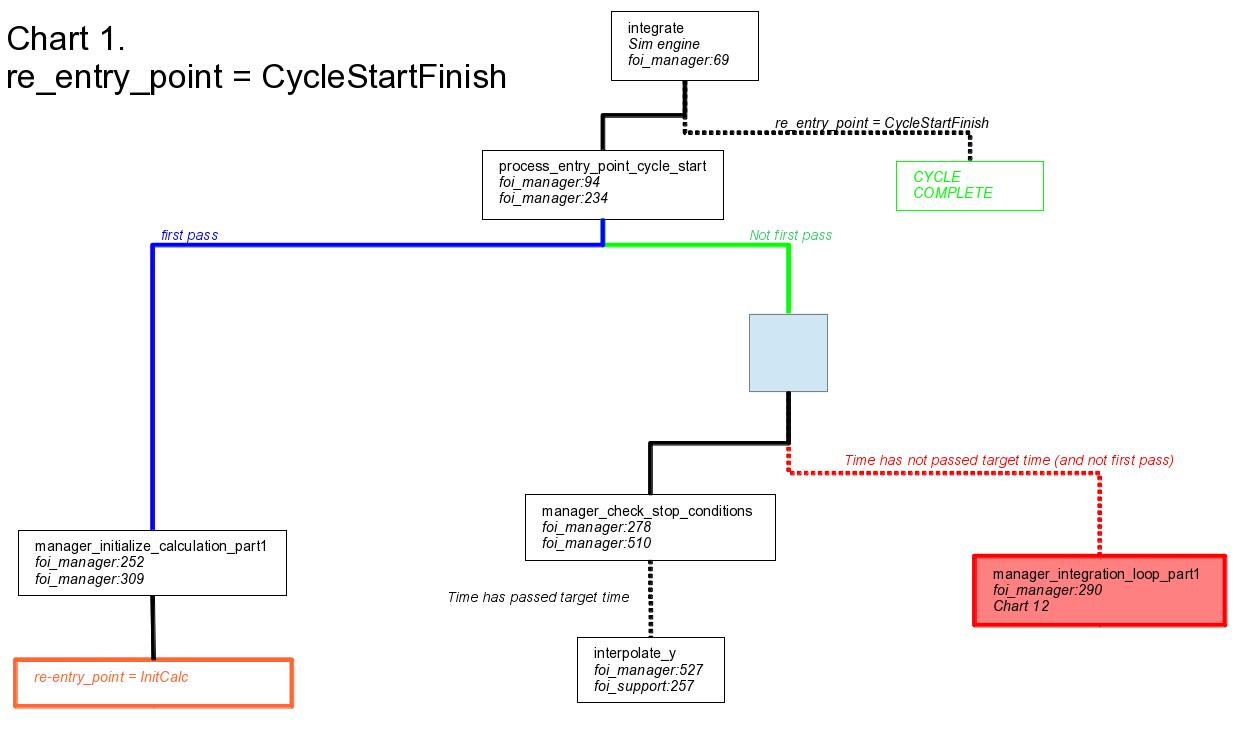
\includegraphics[width=6.5in]{figures/lsode_flow1.jpg}
\caption{Flow Chart 1.}
\end{center}
\end{figure}

\begin{figure}[htp]
\begin{center}
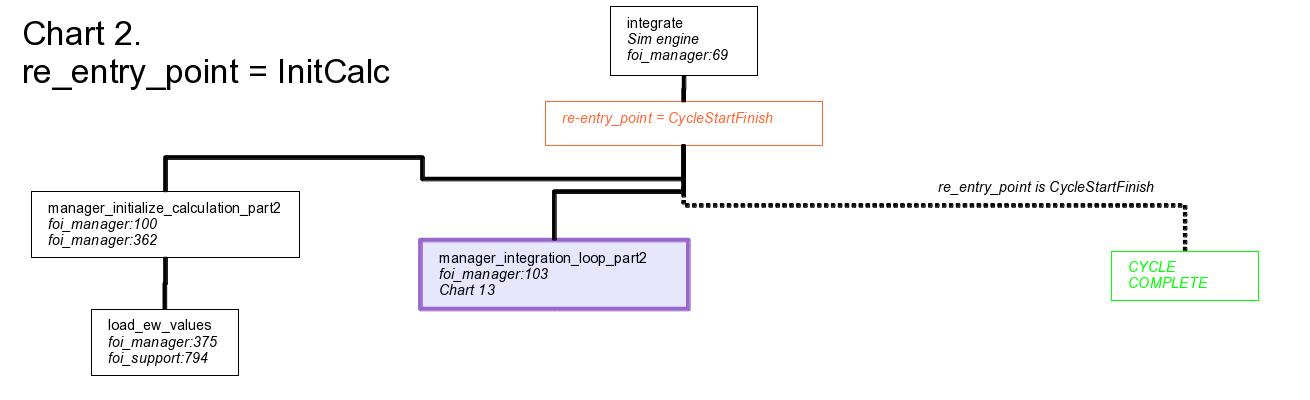
\includegraphics[width=6.5in]{figures/lsode_flow2.jpg}
\caption{Flow Chart 2.}
\end{center}
\end{figure}

\begin{figure}[htp]
\begin{center}
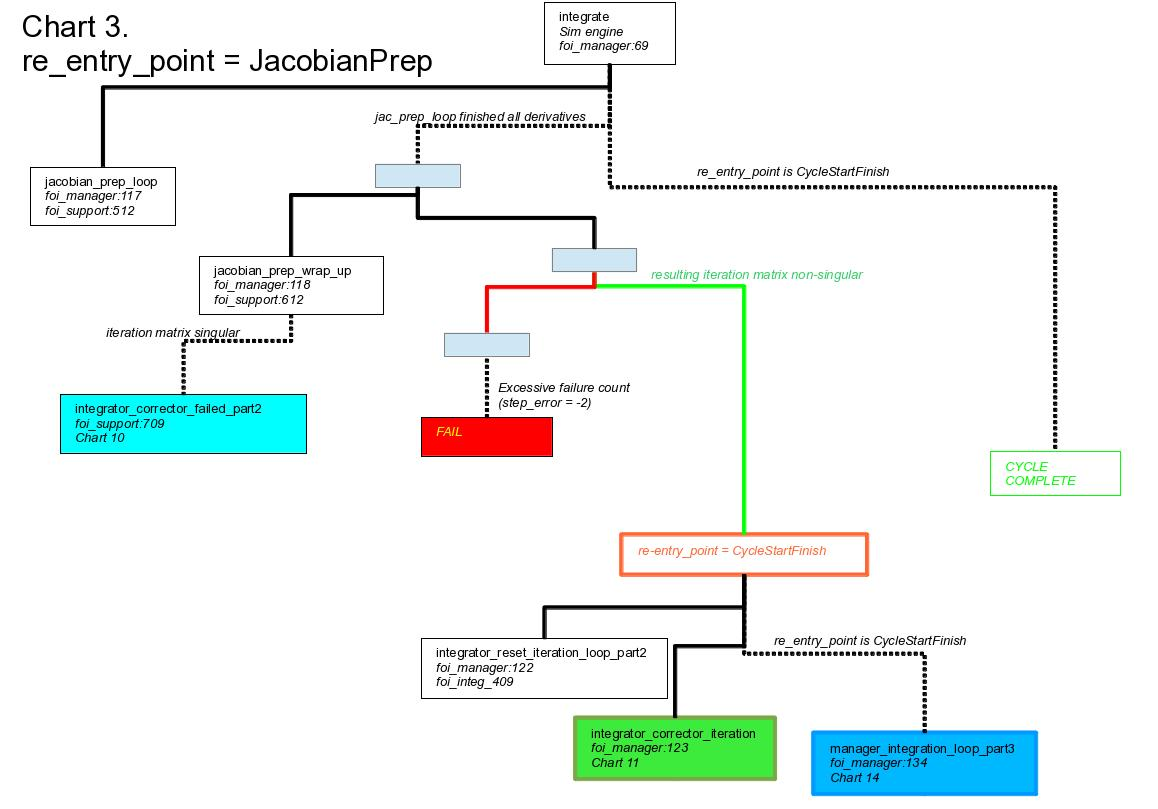
\includegraphics[width=6.5in]{figures/lsode_flow3.jpg}
\caption{Flow Chart 3.}
\end{center}
\end{figure}

\begin{figure}[htp]
\begin{center}
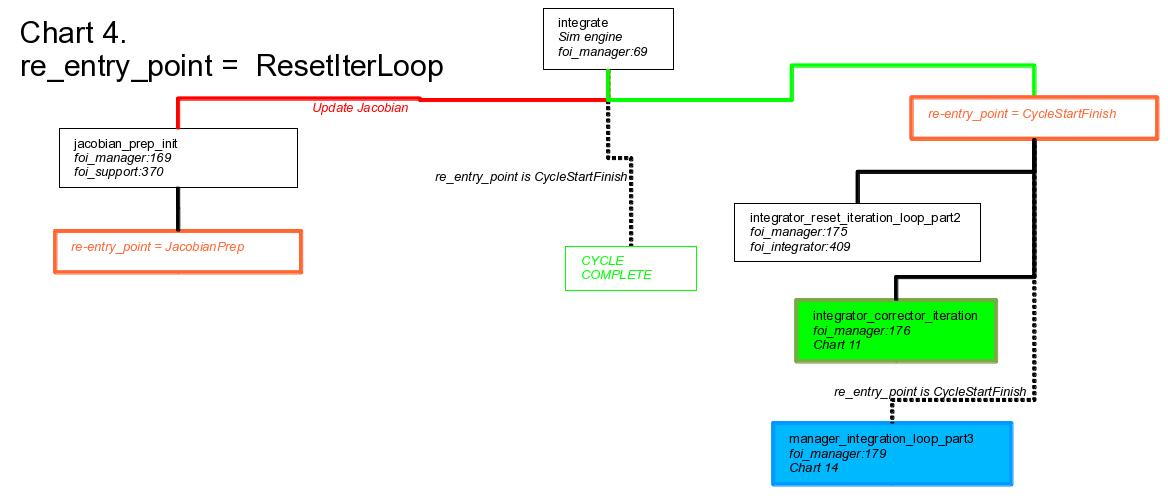
\includegraphics[width=6.5in]{figures/lsode_flow4.jpg}
\caption{Flow Chart 4.}
\end{center}
\end{figure}

\begin{figure}[htp]
\begin{center}
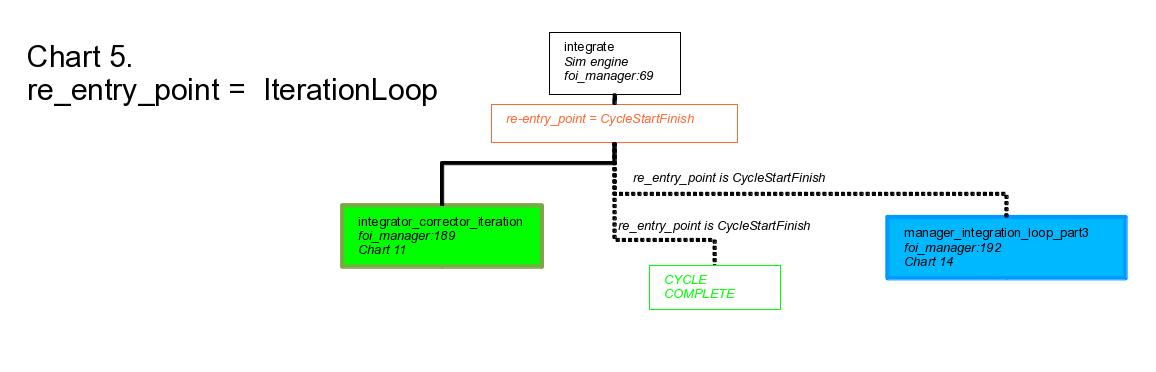
\includegraphics[width=6.5in]{figures/lsode_flow5.jpg}
\caption{Flow Chart 5.}
\end{center}
\end{figure}

\begin{figure}[htp]
\begin{center}
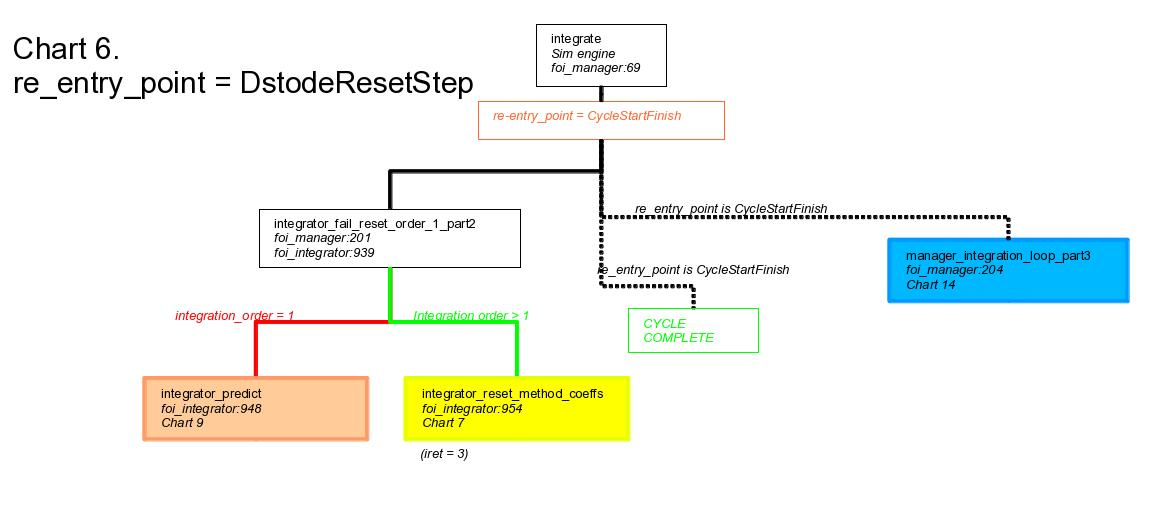
\includegraphics[width=6.5in]{figures/lsode_flow6.jpg}
\caption{Flow Chart 6.}
\end{center}
\end{figure}

\begin{figure}[htp]
\begin{center}
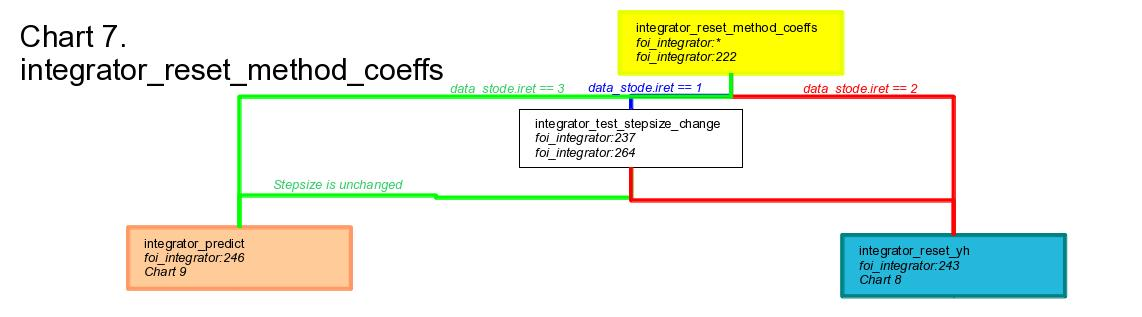
\includegraphics[width=6.5in]{figures/lsode_flow7.jpg}
\caption{Flow Chart 7.}
\end{center}
\end{figure}

\begin{figure}[htp]
\begin{center}
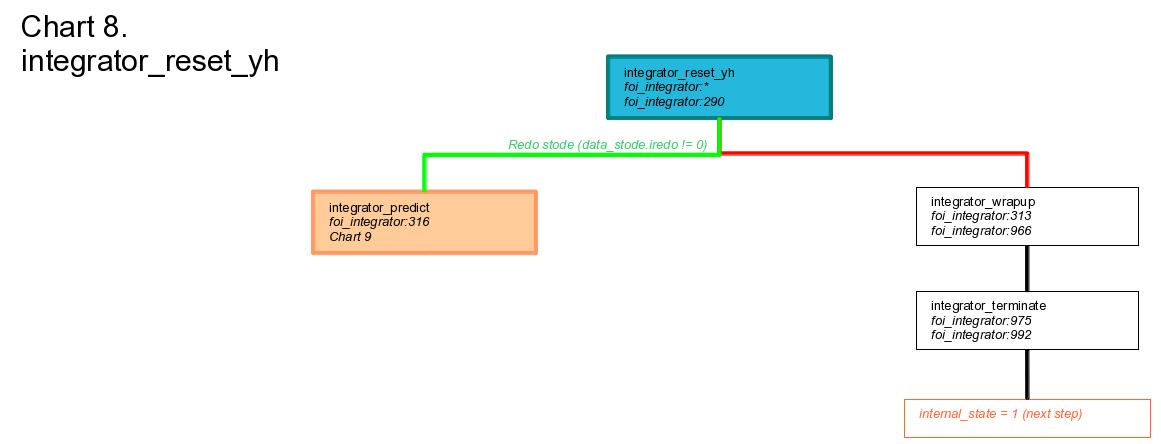
\includegraphics[width=6.5in]{figures/lsode_flow8.jpg}
\caption{Flow Chart 8.}
\end{center}
\end{figure}

\begin{figure}[htp]
\begin{center}
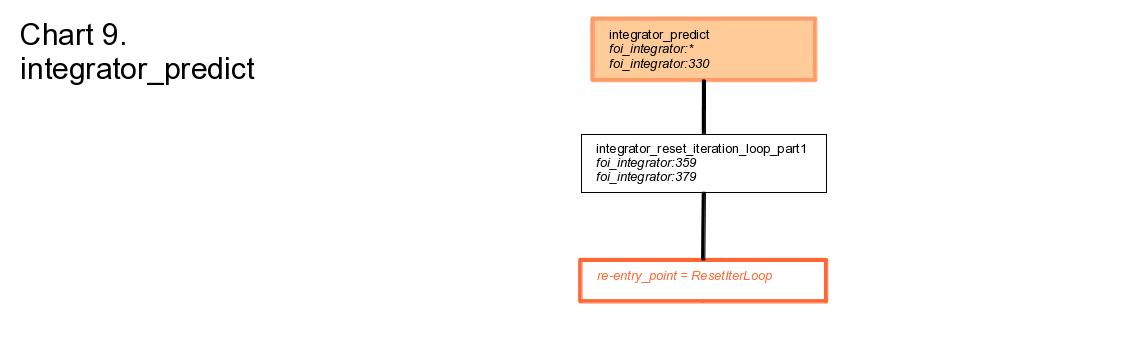
\includegraphics[width=6.5in]{figures/lsode_flow9.jpg}
\caption{Flow Chart 9.}
\end{center}
\end{figure}

\begin{figure}[htp]
\begin{center}
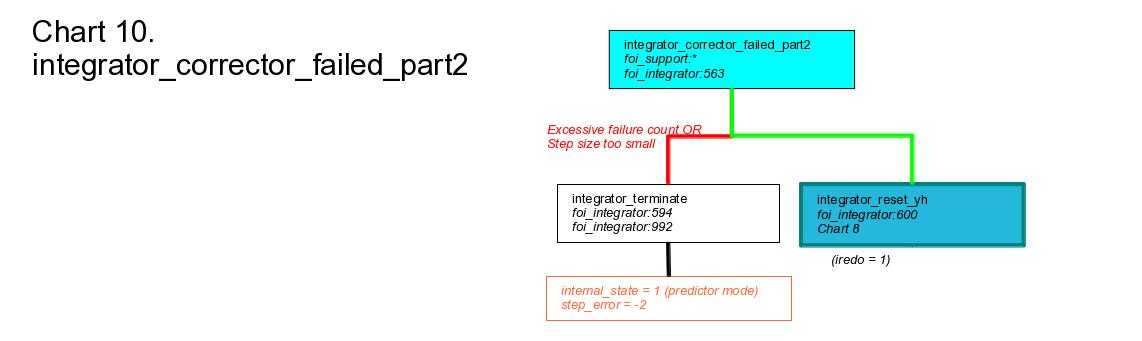
\includegraphics[width=6.5in]{figures/lsode_flow10.jpg}
\caption{Flow Chart 10.}
\end{center}
\end{figure}

\begin{figure}[htp]
\begin{center}
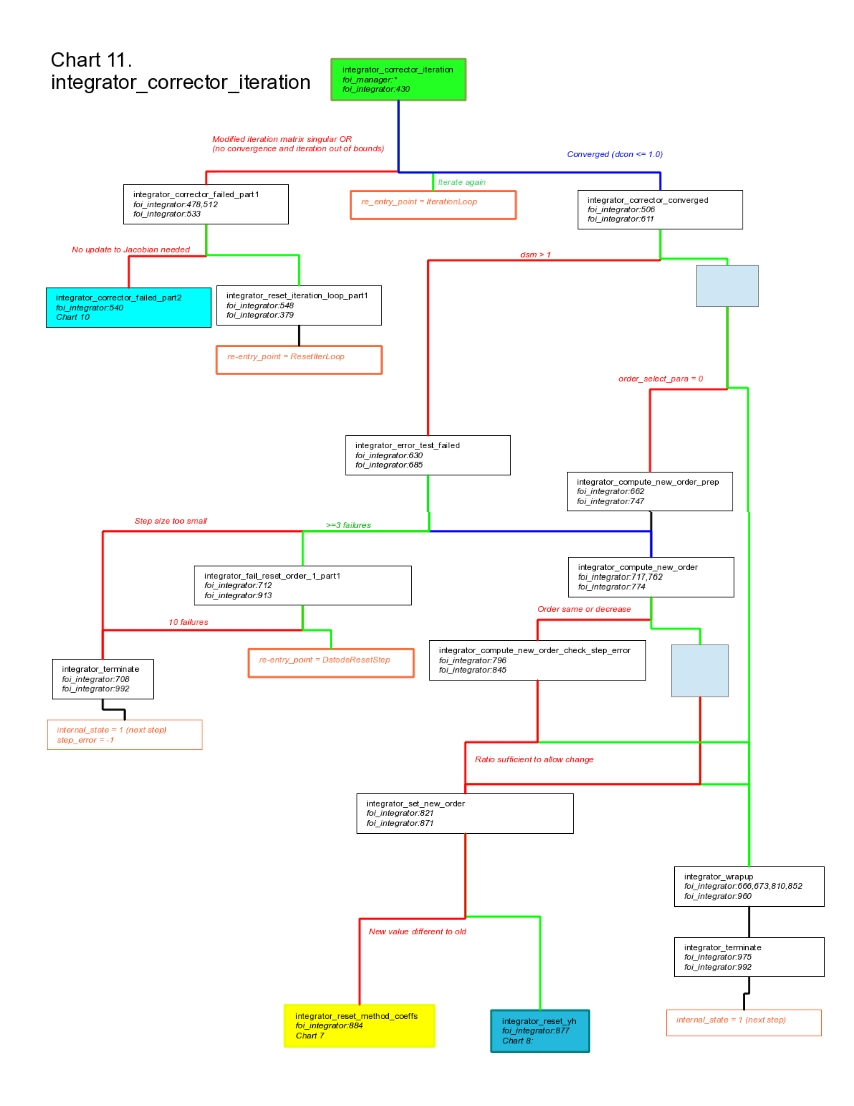
\includegraphics[width=6.5in]{figures/lsode_flow11.jpg}
\caption{Flow Chart 11.}
\end{center}
\end{figure}

\begin{figure}[htp]
\begin{center}
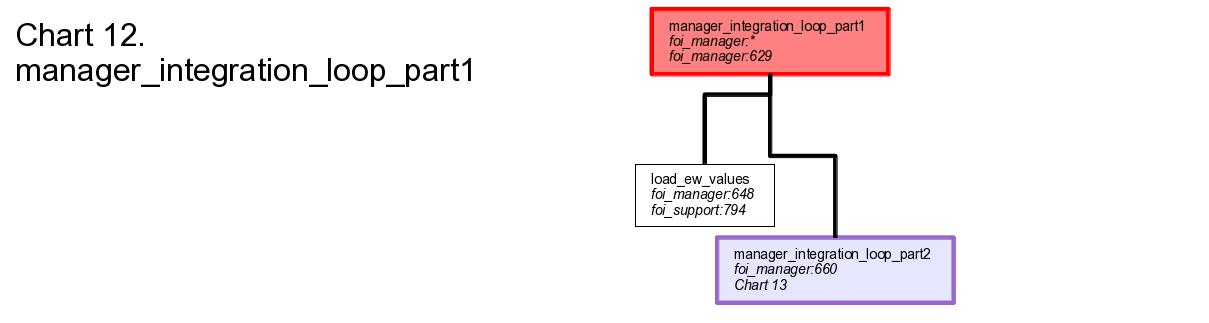
\includegraphics[width=6.5in]{figures/lsode_flow12.jpg}
\caption{Flow Chart 12.}
\end{center}
\end{figure}

\begin{figure}[htp]
\begin{center}
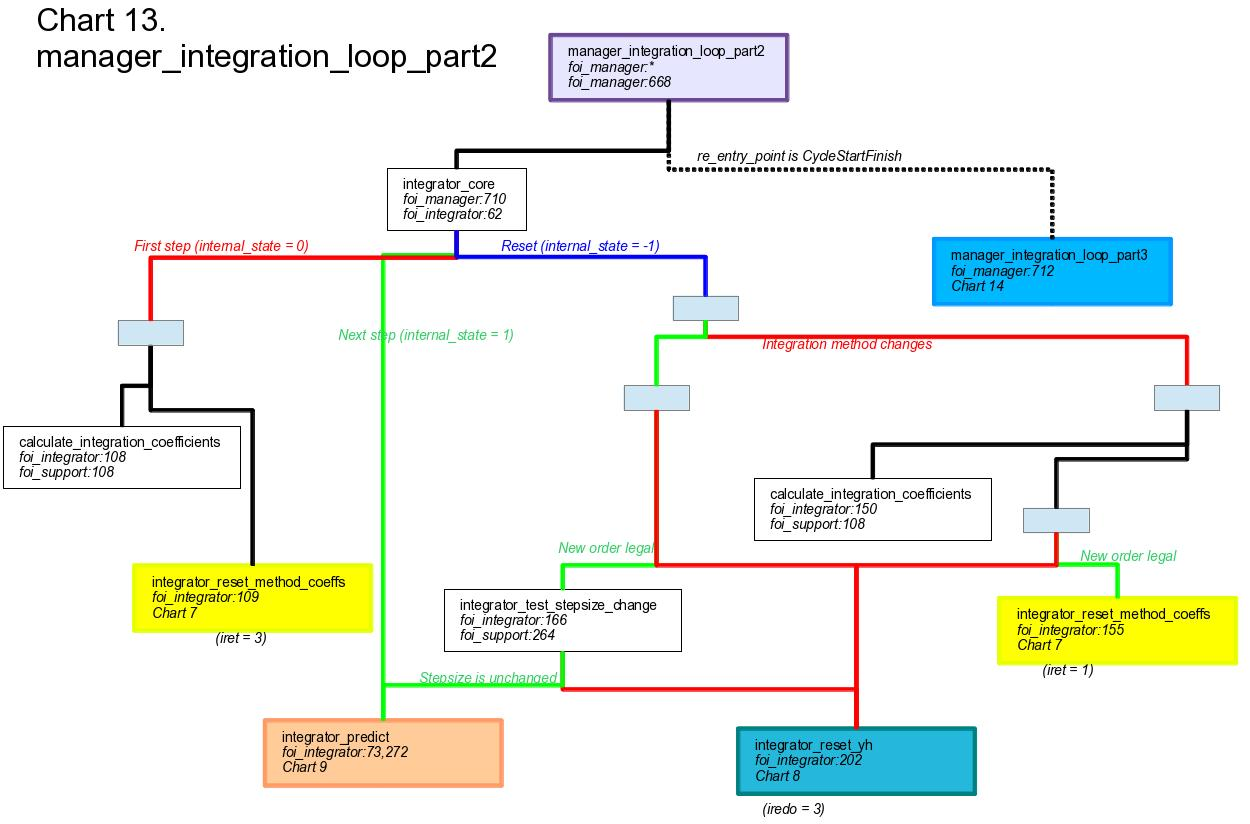
\includegraphics[width=6.5in]{figures/lsode_flow13.jpg}
\caption{Flow Chart 13.}
\end{center}
\end{figure}

\begin{figure}[htp]
\begin{center}
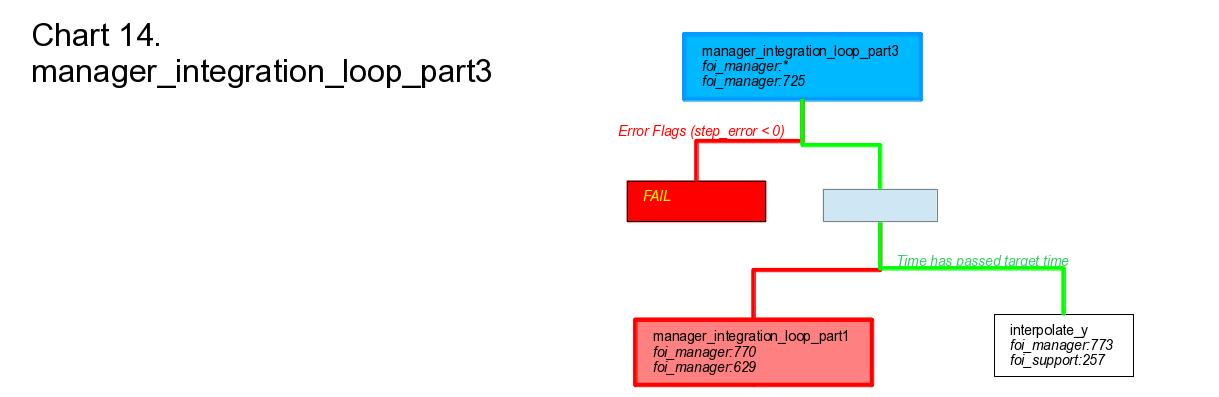
\includegraphics[width=6.5in]{figures/lsode_flow14.jpg}
\caption{Flow Chart 14.}
\end{center}
\end{figure}


\section{First Order ODE}

All LSODE integrations are of first-order equations.  The state vector is
integrated as a single entity, with all components taking the same
time-step and being tested for convergence together.

The LSODE package provides a variable-order, variable-step first-order
integrator.
As each problem initializes, the order starts at one (1) and the step starts
small.  As a history is accumulated, both the order and step-size are
gradually increased automatically.   The order reaches a maximum of 5 or
12, depending on the options chosen; the step-size has no enforced upper bound.

Unlike the other integrators used in JEOD, the time-step for integration is
not enforced from the outside.  The LSODE package determines its preferred
integration step and integrates to that point.  If its integration step
exceeds the target time (dictated from the outside, such as by the simulation
engine), the solution at that target time is interpolated from the history and
the newly created future point.  The next integration cycle continues from the
end of the previous integration step, not from the interpolated point.

It is possible that the internal step-size could grow to exceed the
externally-requested time-step, thereby allowing for the possibility that
multiple target times boundaries could be crossed within one
internal time-step.  In this case, each such target would be iterated from
the generated states, a process that continues until the next target time is
in the future of the last internally generated time.


\section{Second Order ODE}

Second-order equations are treated as a pair of coupled first-order
equations.  The entire state vector (now comprising the zeroth-derivative and
first-derivative values) is integrated as one entity.

\section{Generalized Position / Generalized Velocity ODE}

The LSODE integrator constructor currently does not provide a means
to solve a generalized position / generalized velocity second order ODE.
As such, it is not suitable for integrating rotational state.

\section{Lie Group Second Order ODE}

The LSODE integrator constructor currently does not provide a means
to solve a Lie group (generalized step) second order ODE.

\section{Usage Instructions}

\subsection{Disable Rotational State}

This implementation of LSODE is limited to integrating translational state
only.  It lacks the ability to handle the generalized-position /
generalized-velocity problems associated with integrating rotational state.

To use LSODE to integrate the state of 6-DOF bodies (e.g. bodies of type
\textit{DynBody}), the rotational state must be turned off and the
\textit{three-dof} flag set to true.

\begin{verbatim}
Example:
   vehicle.dyn_body.rotational_dynamics = False
   vehicle.dyn_body.three_dof = True
\end{verbatim}

\subsection{Force Ephemerides Rate High}

The Ephemerides Model Manager (most commonly found as the Dynamics Manager)
contains a flag, \textit{deriv\_ephem\_update}, that indicates whether or not
the
ephemerides update should be performed at the derivative rate (i.e.,
whether or not the planetary positions should be computed at every point in
time corresponding to a computation of the state derivatives).

In most
simulations (including those built following recommended practice from the
pre-packaged
simulation-modules), the ephemerides update is called at the integration
rate.  For most integrators, this is typically a short timescale, on the order
of tens of seconds or less. Consequently, for most scenarios, updating the
planetary positions at the derivative rate is entirely unnecessary and the
default
setting for this flag is \textit{false}.

However, LSODE can handle very large integration steps.
Indeed, since it can take many internal steps per specified time-step, the
specified (external) time-step is really limited only by the maximum
allowable number of internal steps per external step (this is a
user-specified value, see below).  Relying only on the default ephemerides
update to reposition the planets at a pre-determined interval -- that may be
orders of magnitude larger than necessary -- is not a good idea.  Therefore,
when using LSODE, it is \textbf{strongly recommended} that the flag be set.

\begin{verbatim}
    dynamics.dyn_manager.deriv_ephem_update = True
\end{verbatim}

If this step is omitted and the ephemerides updated too sparsely, each planet
will physically “jump” to a new position that is a significant departure from
its old position.  Consequently, the gravitational accelerations experienced
by the vehicle can go through a significant discontinuity.  The resulting
effect in the integrator is quite subtle and easily overlooked.

The prediction of the next state is made based
on the derivative values at the end of the previous internal step, while
the correction calculation is made based on the derivative values at the
start of
the current internal step.  When the derivatives are smooth, these values
differ minimally and convergence can be quickly achieved over very large
time-steps.  When there is a discontinuity in the acceleration, the corrector
adjustments
will not easily converge with the original predictor calculations.  LSODE
will automatically reduce the internal timestep until they do converge.  The
effect is that while the integration step may be hundreds of thousands
of seconds (or larger), the internal step could be limited to
milliseconds (or smaller) to enforce the convergence across the discontinuity.
From there, the internal time-step will be allowed
to grow, but may only reach tens or hundreds of seconds before the next
ephemerides update causes another discontinuity
and the process repeats.  The end result is that the LSODE integrator
will perform very poorly -- both in terms of numerical accuracy and speed --
but it will not fail in any obvious or recognizable way.

A further incidental complication arises with the interpolation of state
to the target time.  Suppose the integrator is to integrate from time
$t_0$ to time $t_1$ and from $t_1$ to $t_2$.  It will probably overshoot to
time $t_1' > t_1$ and interpolate
back to the target time $t_1$.  The next phase of integration will begin
where the previous left off, at $t_1'$ . Thus, the ephemerides data will change
partway through the integration step going from $t_1$ to $t_2$.
The ephemerides data from $t_0$ will
be used for $t_1  < t <  t_1'$ and the data from $t_1$  will be used for
$t_1' < t < t_2$.  This invalidates any comparison to other integrators.

By forcing the ephemerides update to the derivative rate (the fastest possible
rate given the structure of the integrator), control over when the update is
performed passes from the
pre-configured schedule of the simulation engine back to the integrator
itself.  The integrator may, in some cases, be able to handle updates that are
thousands
of seconds apart, but that determination is
better left to the integrator as it computes its own internal step-size.

\subsection{Configuring the Integrator}

There are several options available for configuring the integrator.  These
values are found in the \textit{LsodeControlDataInterface} class, instantiated
within the integrator constructor at \newline
\textit{$<$lsode\_integrator\_constructor$>$.data\_interface}.

\textbf{Two configuration parameters -- the relative error tolerance and
the absolute error tolerance --
must be specified; the others are optional.}

As with other integrators, the constructor is only used in the process
of creating the integrator; changes made to data elements in the constructor
can only be propagated to the integrator when it is constructed.  Additional
changes made after the integrator has been built will be ignored. Thus,
these options are only available at initialization.

For example, for a simulation in which the integrator is specified at the
input-file level, one might find:

\begin{verbatim}
  lsode_integrator = trick.LsodeIntegratorConstructor()
  lsode_integrator.data_interface.set_rel_tol (0, 1.0E-15)
  lsode_integrator.data_interface.set_abs_tol (0, 1.0E-12)
\end{verbatim}


\subsubsection{Error Tolerance}

The allowable error tolerance for an integration process to be considered
converged is a
combination of two factors - an absolute value (that is independent of the
state) and a relative value (that scales linearly with the state).  These
values are combined to give the total error tolerance.  When
subsequent computations produce predictor/corrector values that are within
the total error tolerance of
one another, the integration has converged.

Ideal values for the absolute and relative error tolerances are
problem-specific, and often component-specific.  Hence, it is necessary to
specify these two values for the particular problem at hand.  The default
values are illegal.

One or both must
be non-zero; if both the absolute and relative tolerances are zero, there
is zero permissible deviation, and the integrator can never
converge.

\subsubsection{Absolute Error Tolerance}
\textit{abs\_tolerance\_error\_control\_vec}

\begin{itemize}
\item Type:  double vector; double array.
\item Default: -1.0
\end{itemize}

The absolute error tolerance provides the permissible difference between
subsequent corrector-iterations in order for the corrector to be considered
converged.  \textbf{This value MUST be specified}; the default value is
illegal.  A zero value means that the absolute error will not be considered in
determining the convergence.
Initially, the values will populate the vector
\textit{abs\_tolerance\_error\_control\_vec}.
 Once complete, these values will be copied into an appropriately-sized
allocated array, \newline \textit{abs\_tolerance\_error\_control}.
The method \textit{set\_abs\_tol} should be used to populate these values.
This method takes 2 arguments, the index and the value.
\begin{verbatim}
  lsode_integrator.data_interface.set_abs_tol(index,value)
\end{verbatim}
Notes:
\begin{itemize}
\item
No units are specified for this value.  The specified value assumes the
default units for the variable to which it is being applied.  When
integrating an orbital body, that is meters for position and
meters-per-second for velocity.
\item
If using a common specification for all absolute tolerances (see Error
Control Indicator below), only one
value is needed; it must be input at index 0.
\item
All specified values must be non-negative.
\item
If an entry is made at index n ($n>0$) then all non-specified values at prior
indices ($i<n$) default to -1.0 and must be specified before continuing.
\item
If selecting options \textit{SpecificAbs*} (see Error Control Indicator
below), unspecified entries at indices higher
than the highest specified index default to 0.0 and no check is made that
values have been input for these components.
\item
An absolute error tolerance of 0.0 is legal, but dangerous.  If one of
the state components happens to be extremely close to 0, the relative
error will be consequentially small, and the allowable error may be too
small for the machine to handle.  Absolute error tolerances should be
greater than 0.0 unless the user is absolutely confident that their state
component(s) can never go to zero.
\item
In the absence of a legitimate value, use something small, such as
$10^{-12}$.
\end{itemize}


\subsubsection{Relative Error Tolerance}
\textit{rel\_tolerance\_error\_control\_vec}

\begin{itemize}
\item
Type:Vector, double; double array.
\item
Default: -1.0
\end{itemize}
The relative error tolerance provides the permissible difference between
subsequent corrector-iterations – as a fraction of the state itself –
in order for the corrector to be considered converged.  \textbf{This value MUST
be specified}; the default value is illegal.  A zero value means that the
relative error will not be considered in determining the convergence.
Initially, the values will populate the vector 
\textit{rel\_tolerance\_error\_control\_vec}.
 Once complete, these values will be copied into an appropriately-sized
allocated array, \textit{rel\_tolerance\_error\_control}.
The method \textit{set\_rel\_tol} should be used to populate these values.
This method takes 2 arguments, the index and the value.
\begin{verbatim}
  lsode_integrator.set_rel_tol(index,value)
\end{verbatim}
Notes:
\begin{itemize}
\item
If using a common specification for all relative tolerances, only one
value is needed; it must be input at index 0.
\item
All specified values must be non-negative.
\item
If an entry is made at index n ($n>0$) then all non-specified values at prior
indices ($i<n$) default to -1.0 and must be specified before continuing.
\item
If selecting options \textit{*SpecificRel}, (see Error Control Indicator
below) unspecified entries at indices higher
than the highest specified index default to 0.0 and no check is made that
values have been input for these components.
\item
An absolute error tolerance of 0.0 is legal, but dangerous.  If one of
the state components happens to grow large, the relative error associated
with a small absolute error against a large state may be too small for
the machine to handle.  For example, an absolute tolerance of $10^{-12}$ on
a state with a value of $10^6$ is only one part in $10^{18}$, which demands
precision
that exceeds the capability of a double-precision value.  Such an absolute
error loses all significance and is effectively zero.  Relative error
tolerances should be greater than 0.0 unless the user is absolutely confident
that the specified absolute tolerance will always be significant across
the entire range of the possible state.
\item
In the absence of a legitimate value, use something close to the limit of
resolution of a double precision, such as
$10^{-15}$ (i.e. one part in $10^{15}$).
\end{itemize}


\subsubsection{Error Control Indicator} \textit{error\_control\_indicator}
\begin{itemize}
\item Type: ErrorControlIndicator
\item Options:
 \begin{enumerate}
 \item CommonAbsCommonRel
 \item SpecificAbsCommonRel
 \item CommonAbsSpecificRel
 \item SpecificAbsSpecificRel
 \end{enumerate}
\item Default:  CommonAbsCommonRel   (1)
\end{itemize}

Each integration cycle completes when the corrector-phase produces a result
that is within some specified tolerance of the previous corrector result.
 The tolerances must be specified to be either (or both) relative to the
state (e.g. 1 part in $10^{12}$) or an absolute discrepancy of default units
(e.g. within  $10^{-9} m$).  These tolerances can also be specified to be
applied
commonly across all components, or with a specific value for each component.
Note that in the case where different state components have different units
(e.g. position and velocity in a 6-vector), the numerical value for the
absolute error tolerance will be interpreted as being expressed in the
default units of the variable (in this case, $m$ and $m s^{-1}$).

This control flag indicates which of these options to choose.
Specification of the tolerance values is covered in the two sections
immediately preceding.
\begin{enumerate}
\item \textbf{CommonAbsCommonRel} \newline
Apply a common absolute tolerance and common
relative tolerance to all components.
\item \textbf{SpecificAbsCommonRel}  \newline
Apply a per-axis absolute tolerance and a
common
relative tolerance.
\item \textbf{CommonAbsSpecificRel}  \newline
Apply a common absolute tolerance and a
per-axis relative tolerance.
\item \textbf{SpecificAbsSpecificRel} \newline
Apply a per-axis absolute tolerance and
another per-axis relative tolerance.
\end{enumerate}



\subsubsection{Number of ODEs}
\textit{num\_odes}

\begin{itemize}
\item
Type: unsigned int
\item
Default: 3, set to 6 for integration of a \textit{Simple6DofDynBody}
\end{itemize}
This values specifies the number of ODES in the system to integrate.
Note that this option is invalid when using LSODE for the JEOD's default
purpose of integrating vehicle state.  The creation of the integrator
for that purpose will automatically assign this value to six (three
position and three velocity values).

\subsubsection{Integration Method}
\textit{integration\_method}

\begin{itemize}
\item
Type:IntegrationMethod
\item
Options:
\begin{enumerate}
\item
ImplicitAdamsNonStiff
\item
ImplicitBackDiffStiff
\end{enumerate}
\item
Default:ImplicitAdamsNonStiff
\end{itemize}
The integration\_method determines which integration algorithm to use.
For stiff problems, the ImplicitBackDiffStiff option should be chosen.
Most orbital problems are not considered stiff and the default to use
is the ImplicitAdamsNonStiff.
The maximum order is 12 for the ImplicitAdamsNonStiff method, and 5 for
the ImplicitBackDiffStiff method.

\subsubsection{Corrector Method}
\textit{corrector\_method}

\begin{itemize}
\item
Type:CorrectorMethod
\item
Options:
\begin{enumerate}
\setcounter{enumi}{-1}
\item
FunctionalIteration
\setcounter{enumi}{1}
\item
NewtonIterInternalJac
\item
JacobiNewtonInternalJac
\end{enumerate}
\item
Default: FunctionalIteration
\end{itemize}
The \textit{corrector\_method} determines which algorithm to use for the
corrector-phase of the integration.
FunctionalIteration is the simplest and the default.
NewtonIterInternalJac uses a modified Newton iteration scheme utilizing
an internally generated numerical Jacobian
JacobiNewtonInternalJac uses a modified Jacobi-Newton iteration scheme
utilizing an internally generated numerical Jacobian
Note that options 1, 4, and 5 (modified Newton iteration with user-supplied
Jacobian, with user-supplied banded Jacobian, and with an internally generated
banded Jacobian) are not supported in this implementation.



\subsubsection{Minimum Step Size}
\textit{min\_step\_size}

\begin{itemize}
\item
Type: double
\item
Default: 0.0
\end{itemize}
For users for whom keeping the simulation ticking over is more important
than precision, there is the option of specifying a minimum step size.
 Note that this represents the minimum absolute value of the step size;
for simulations with negative step sizes, this would still be a positive
value (and would represent the least-negative step size).
The growth of the step-size is a non-trivial process.  When the integrator
starts a problem, the step-size is typically small.  Every few steps,
the step-size is re-evaluated along with the integration order.  A step
size ratio (new step-size / old step-size) is computed for each of 3 cases:
\begin{enumerate}
\item the integration order decreases,
\item the integration order is held constant,
\item the integration order increases.
\end{enumerate}
Whichever order change produces the largest step-size increase is adopted.
 The corresponding step-ratio is compared against that which would be
required to reach the user-specified minimum step-size (this parameter),
and the larger of the two selected (step omitted if no minimum step-size
is input).  Finally, the step-ratio is limited to be no greater than 10.0.
The most challenging convergence problems associated with the usage of
this parameter appear to occur during integrator start-up.  These problems
tend to occur when the step-size growth is forced by the minimum step-size
parameter and when it is significantly larger than the computed ideal
ratio.

For example, consider an initial step-size of 0.1s, a specified minimum
of 20.0s, and a computed ratio of 4.2.  The next ideal step-size would
be 0.42s, the external value of 20.0s is greater, so this takes precedence.
 The 10.0 limit on the ratio ultimately forces the next time-step to 1.0
s, but that is still significantly larger than the ideal step-size.  This
may have problems converging.
Do not misinterpret this parameter as a preferred step size, particularly
for the case of establishing LSODE as a long-arc integrator.  While it
may be desirable to have a large step size for long-arc integration, it
would not be a good idea to specify that value as the minimum step-size.
 Use this parameter carefully.
\subsubsection{Maximum Step Size}
\textit{max\_step\_size}

\begin{itemize}
\item
Type: double
\item
Default: 0.0
\end{itemize}
For systems with states that are easily predictable very far into the
future (e.g. systems with constant gradients) the step sizes can grow
extremely large.  If it is desirable to maintain the step size closer
to the requested step size and avoid extensive interpolation, this option
can be used.
The default value for this parameter is 0.0, but that is interpreted as
infinity.  Any non-zero value will be interpreted as specified.
This parameter is relatively safe to use but can lead to a lack of accuracy.
 By forcing the time-step to be somewhat arbitrarily small, more integration
steps are taken than necessary and numerical error could be increased.
 However, the problems with convergence that frequently interfere with
setting the minimum step-size are unlikely to be encountered as a result
of setting this parameter.
\subsubsection{Initial Step Size}
\textit{initial\_step\_size}

\begin{itemize}
\item
Type: double
\item
Default: None
\end{itemize}
This is the very first time-step to try.  If not specified, a value will
be computed.
There are some overriding safeguards on this value, and the internal
error-checking
often makes setting this value redundant anyway.  If the value is too
high for the integrator to converge, the integrator will reduce the step-size
automatically until it is suitable for convergence.  After convergence,
if the integrator fails to meet the error checks, the entire time-step
(based on the user-specified value) will be discarded and the integrator
will return to its previous safe value; this is normal operating practice.
 In the case of the first step, the previous safe value is 0.0 and the
integrator will generate its own time-step, just as it would have done
without this value being set.

Without this value being set, the integrator will err on the side of
caution and the initial time-step will tend to be too
small.  However, it will grow by a factor of 10 at each correction until
it reaches
a more suitable value, a process that tends to be completed relatively
quickly.

Setting this parameter would only be useful if:
\begin{itemize}
\item
the user knows, a priori, a suitable value for the starting time-step (i.e.,
a time-step that allows the integrator to converge without error), and
\item
the specified initial time-step is significantly larger than the value
that the integrator would start with, and
\item
the user is planning on running a large number of simulations using
that value where each simulation is very short so that the initialization
time is a significant fraction of the overall simulation time.
\end{itemize}

If any of these conditions are not met, setting this parameter is unlikely
to have any noticeable and beneficial effect.


\subsubsection{Maximum Order}
\textit{max\_order}

\begin{itemize}
\item
Type: unsigned int
\item
Default: 12
\end{itemize}

This is the maximum order allowable for the integrator.  The order starts at
1 and generally increases until it reaches either:
\begin{itemize}
\item The user-specified maximum order (this value) or
\item The maximum-allowable order for the integration method (see 
\textit{integration\_method})
\end{itemize}
Specifying a \textit{max\_order} value greater than the allowable order for
the integration method is completely
redundant.

The safe time-step used by a lower order integrator is smaller than that
for a higher order integrator.  Consequently,  setting this value to less
than the maximum order for the integration algorithm will result in more
steps being taken, slowing down the simulation.  Reducing the order is
unlikely to have any beneficial performance effects.  Unless the user
has a specific purpose for limiting the order (e.g. to compare the performance
of two 8th order integrators), this parameter should probably not be set.


\subsubsection{Maximum Number of Small-step Warnings}
\textit{max\_num\_small\_step\_warnings}

\begin{itemize}
\item
Type: unsigned int
\item
Default:10
\end{itemize}
Occasionally, the integrator may get into a situation in which the step
size it can take is so small that it is effectively zero.  In this case,
the integrator will back up to a previous state and try again.  On each
of these occassions, a warning will be sent to the output that the step
size has become too small.  If the integrator keeps getting stuck, it
is possible that hundreds of these messages could be sent.  This parameter
limits the number of such messages.  After this number is exceeded, the
integration will still proceed; it only shuts off the publishing of the
warnings.

\subsubsection{Maximum Number of Corrector-Iterations}
\textit{max\_correction\_iters}

\begin{itemize}
\item
Type:unsigned int
\item
Default: 3
\end{itemize}
This is the number of times the corrector can be called before either:
\begin{itemize}
\item
convergence must have been achieved, or
\item
the integration step fails.
\end{itemize}

Convergence tends to be achieved very quickly for orbital problems.  Increasing
this value is unlikely to have any noticeable effect.
Note that convergence in this context indicates only that the last application
of the corrector algorithm did not appreciably alter the state from the
previous application of either the predictor or corrector algorithm.
There are two easily confused reasons why the integrator fails to reach
a stable target:
\begin{enumerate}
\item It fails to converge within the maximum number of iterations
\item The real solution is too far from the original predicted solution.
\end{enumerate}

Once the corrector has converged, the accumulated effect of the corrector
applications for this integration step is compared against the tolerance
limits.  If this is too high, the result is still considered unreliable
and discarded.  This latter test is unaffected by this parameter and it
is highly unlikely that changing this parameter will `fix' a failure indicated
by the latter test.


\subsubsection{Maximum Usage for a Jacobian}
\textit{max\_num\_steps\_jacobian}

\begin{itemize}
\item
Type: unsigned int
\item
Default:20
\end{itemize}
This provides the maximum number of steps that can be taken with a given
Jacobian matrix.  For slowly-evolving systems with short time-steps, this
number may be large.  For rapidly evolving systems, it should be small.
Note that this parameter is redundant if the \textit{corrector\_method} is
\textit{FunctionalIteration}
because the Jacobian us not used for that process.


\subsubsection{Maximum Number of Convergence Failures}
\textit{max\_num\_conv\_failure}

\begin{itemize}
\item
Type:unsigned int
\item
Default:10
\end{itemize}
If the corrector does not converge within \textit{max\_correction\_iters}
iterations,
it is considered failed and the integrator will back up and try again
with a different (smaller) step size.  If it continues to fail, doing
so this many times, then the integrator itself is considered to have failed
to reach the target and the integration stops.

\subsubsection{Maximum Number of Steps}
\textit{max\_num\_steps}

\begin{itemize}
\item
Type:unsigned int
\item
Default:500
\end{itemize}
In the integration of any problem, LSODE will try to reach or exceed the
target time in some number of time-steps, where the time-steps are computed
internally and iterated until the integrator converges within its limits
on each step.  This parameter specifies the largest number of steps that
the integrator can take in solving a particular problem.

For example, suppose the simulation engine called for an integration over
a 60-second interval and the integrator tried steps of 1s, 2s, 2.5s, 4s,
8s, 12s, 10s, 15s, 14s, ... .  Summing these values indicates that the
integrator has passed its first target of 60 seconds in 9 steps. If the user
had stipulated that the integration had to be reached in no more than
\textit{max\_num\_steps = 5} steps, then the integration would have failed
at 17.5s.

The step-count is incremented throughout the entire simulation, but with
each new call to the integrator (a new call is one with
\textit{re\_entry\_point
= CycleStartFinish}), the step-count at step-start is reassigned. Then
the step-count for comparison against \textit{max\_num\_steps} is the
difference
between the step-count for the simulation and the step-count at step-start.

